\documentclass[a4paper,11pt]{jsarticle}

% ===== パッケージ =====
\usepackage[top=25mm,bottom=25mm,left=20mm,right=20mm]{geometry}
\usepackage[dvipdfmx]{graphicx}
\usepackage[dvipdfmx]{pdfpages}
\usepackage{amsmath, amssymb}
\usepackage{setspace}
\usepackage{caption}
\usepackage{url}
\usepackage{titlesec}
\usepackage{abstract}
\usepackage{cite}
\usepackage{booktabs}

% ===== 日本語キャプション =====
\captionsetup[figure]{labelsep=space,labelfont=bf,name=図}
\captionsetup[table]{labelsep=space,labelfont=bf,name=表}

% ===== セクション体裁 =====
\titleformat{\section}{\large\bfseries}{\thesection.}{0.5em}{}
\titleformat{\subsection}{\normalsize\bfseries}{\thesubsection}{0.5em}{}

% ===== 行間 =====
\setstretch{1.2}

% ===== タイトル情報 =====
\title{研究室配属レポート題目}
\author{氏名:山田 太郎\\学籍番号:12345678\\所属:○○大学医学部 ○○研究室\\指導教員:○○教授}
\date{\today}

\begin{document}

% ===================================
% PDF表紙を挿入
% ===================================
\onecolumn
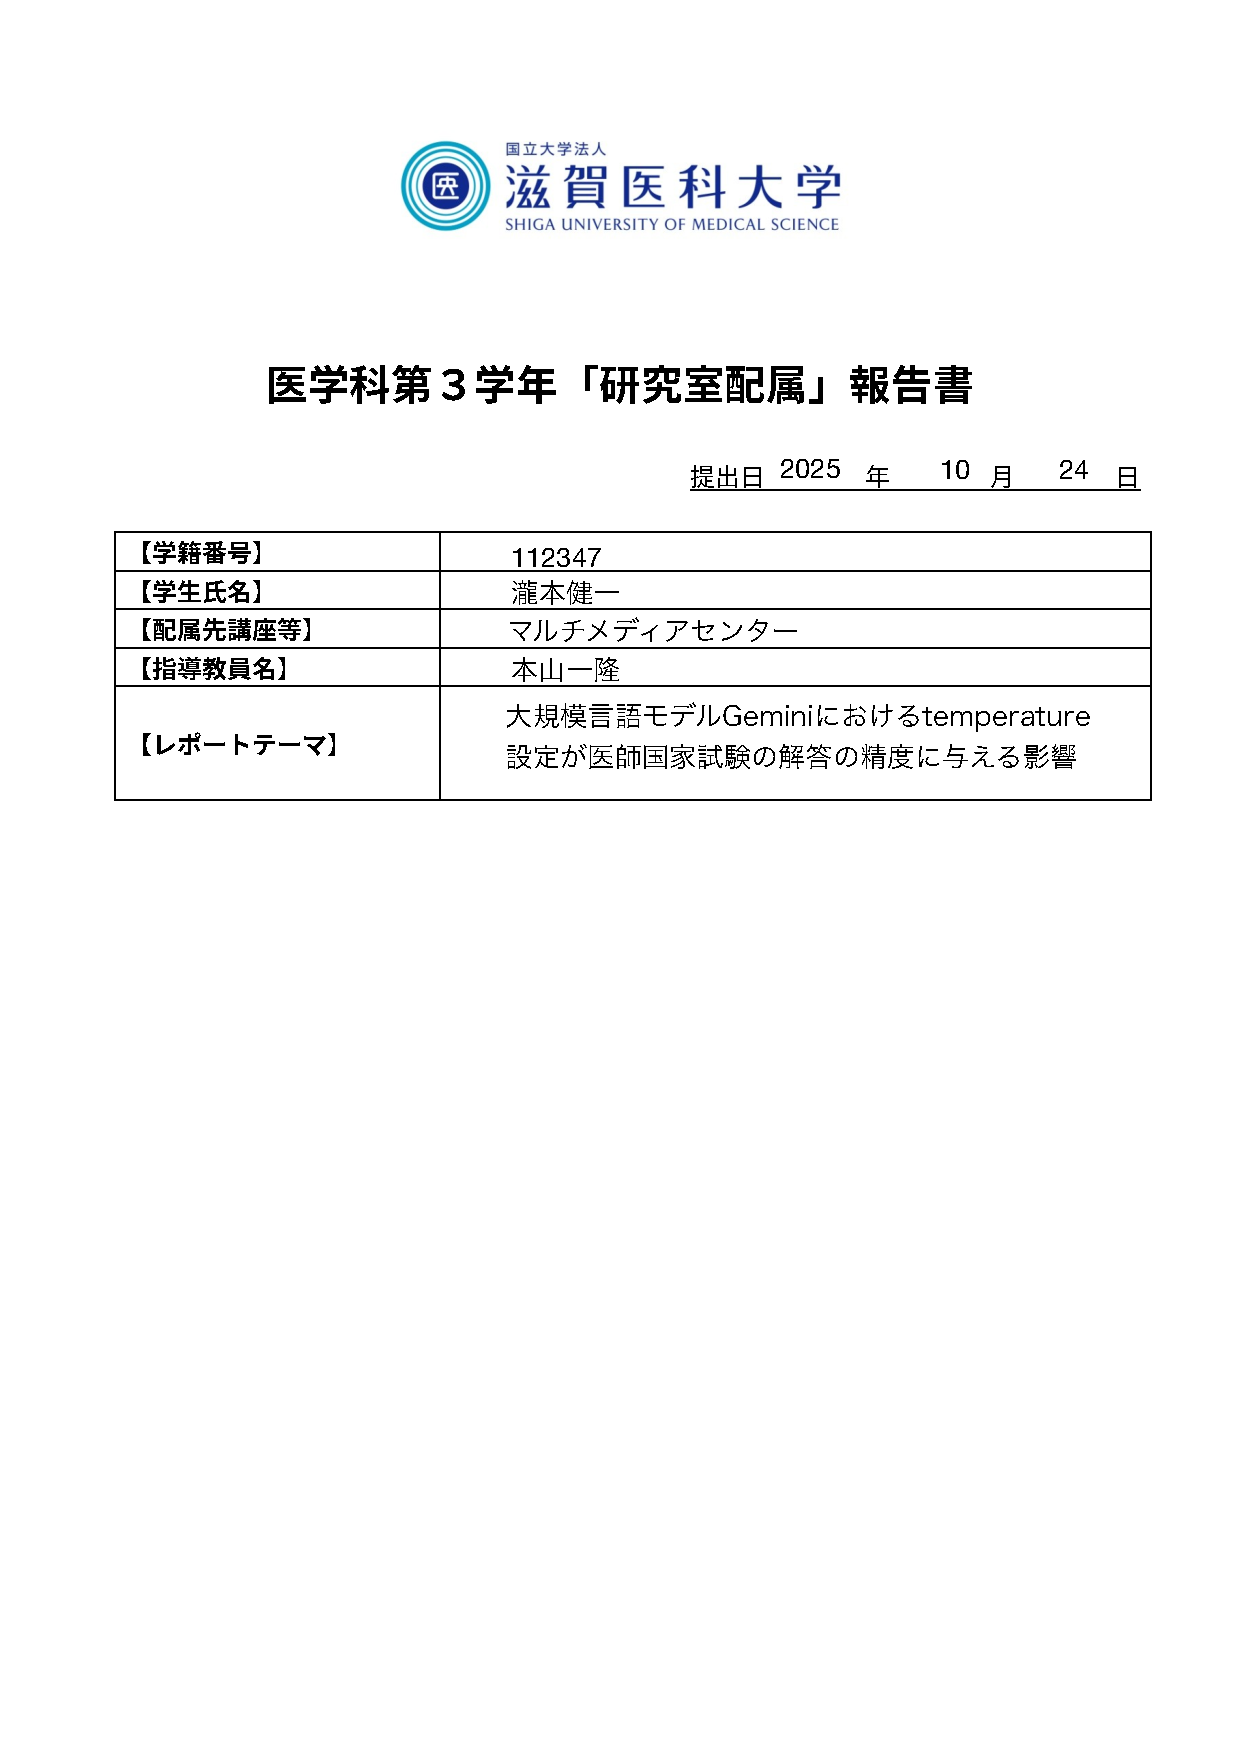
\includepdf[pages=-,pagecommand={},fitpaper=true]{cover.pdf}
\newpage

% ===================================
% 要旨(1段組)
% ===================================
\begin{abstract}
本研究では,大規模言語モデルGeminiを用い,\ temperature設定の違いが医師国家試験問題に対する解答性能に与える影響を検討した.第118回の医師国家試験問題のA問題のPDFから問題文を抽出し,\ temperatureを0.2,\ 0.4,\ 0.6,\ 0.8,\ 1.0の各値に設定してGeminiに回答させた.また,プロンプトは2種類用意した.各回答について正答率および出力内容の一貫性を評価した結果,\ temperatureが低い条件では回答の安定性が高かった.一方,temperatureを高く設定すると,回答のフォーマットに多様性がみられるようになったものの,正答率に大きな変化はみられなかった.これらの結果は,医師国家試験レベルの問題において,\ Geminiの回答がtemperature設定に対して比較的頑健であることを示唆するものである.
\end{abstract}

% ===================================
% 本文
% ===================================
\section{序論}
近年,大規模言語モデル(Large Language Model, LLM)の発展により,人工知能が自然言語処理だけでなく,教育・医療分野での応用も注目されている.特に,医師国家試験のような高難度の専門知識を要する問題に対して,\ LLMがどの程度正確に解答できるかは,AIの教育的利用や学習支援の可能性を評価する上で重要な指標となる.

LLMの出力は,生成アルゴリズムのパラメータによって変動することが知られている.その中でも,\ temperatureは生成のランダム性や多様性を調整する主要なハイパーパラメータであり,低い値では決定的な出力,高い値では多様な応答が生成されるとされる.

本研究では,\ LLMの一つであるGeminiを対象に,複数のtemperature設定における医師国家試験問題への回答精度を比較し,出力の安定性や正答率への影響を評価することを目的とする.

\section{方法}
本研究では,大規模言語モデルGemini-2.0-flashを用いて,医師国家試験問題への回答性能を評価した.実験環境はGoogle Colab上で構築し,Pythonを用いてAPI経由でモデルを呼び出した.

対象とした問題は,厚生労働省が公表している医師国家試験のA問題PDFから,Colab上で文字列として抽出した.抽出にはPythonのPDF解析ライブラリを使用し,選択肢と問題文を適切に整形した.

プロンプトは2種類用意し,各プロンプトに対してtemperatureを0.2から1.0まで,0.2刻みで設定した.各条件において,モデルは5回ずつ回答を生成した.これにより,temperatureとプロンプトの組み合わせごとの回答傾向や正答率の変動を比較可能とした.

実験に用いたソースコードはGitHub上で公開しており,以下のリンクから参照可能である:
\url{https://github.com/ユーザー名/リポジトリ名}

必要に応じて,本レポート中にもソースコードの一部を掲載し,モデル呼び出し例やプロンプトの設定方法を示した.
例えば,Pythonによるモデル呼び出しは以下のように記述した:

\begin{verbatim}
import openai

response = openai.chat.completions.create(
model="gemini-2.0-flash",
messages=[{"role":"user","content":prompt}],
temperature=temp
)
\end{verbatim}

このようにして,temperatureの異なる条件で得られた回答を収集し,正答率および出力内容の傾向を比較分析した.

\section{結果}
図や表を用いて結果を明示する(例:図\ref{fig:example}).

\section{考察}
結果の解釈を述べる.先行研究との比較,考えられる機序,研究の限界などを整理する.

\section{結論}
研究の主な結論を1~3文程度で明確に述べる.

\section*{謝辞}
指導教員や協力者への謝辞を簡潔に記す.

\begin{thebibliography}{9}
\bibitem{ref1} 山田太郎ほか.○○に関する研究.日本医学会誌.2023; 112(4): 123–130.
\bibitem{ref2} Smith J, et al. Analysis of ○○. J Med Sci. 2022; 45(2): 200–210.
\end{thebibliography}

\end{document}
